

\input{../Latex_Templates/Preamble_Report}

%%%%% TITLE PAGE

%\subject{, VT23}
\title{ Report for the Course Modelling in Computational Science, HT23 \\[1ex]
	  \large Project 1: The Potts model}
%\subtitle{}
\author{Theo Koppenhöfer}
\date{Lund \\[1ex] \today}

\addbibresource{bibliography.bib}

\usepackage{pythonhighlight}
\graphicspath{{../Figures/}}

%%%%% The content starts here %%%%%%%%%%%%%


\begin{document}

\maketitle

\section{Introduction}

The following report is part of the first project of the Modelling in Computational Science course at Lund University, HT2023.
In the first project we implemented a Monte-Carlo simulation of the $q$-state Potts model.
The report and the Python implementation can be found online under \cite{Repository}

\section{The Potts model}

A state of the $q$-state Potts model of a $L\times L$ flat grid is given by a mapping
\begin{align*}
	s\colon \brk[c]{1,\dots,L}\times\brk[c]{1,\dots,L}\to\brk[c]{1,\dots,L}\,.
\end{align*}
One assigns this state an energy via
\begin{align*}
	E = -J\sum_{\substack{i, j\text{ neighbouring}\\ \text{grid points}}}\delta\brk*{s_i,s_j}
\end{align*}
where $\delta$ denotes the Kronecker-delta and $J=1$ is the coupling strength. As given in the problem setting we assume periodic boundary conditions on the grid.

\section{The implementation}

\subsubsection{Determining when the Energy has plateaued}

The energy of the system takes some time $t_0$ to reach an equilibrium state. To determine $t_0$ we calculate in every step $i$ moving averages $\text{ma}_1$ and $\text{ma}_2$ over $n$ energies. The construction is shown in figure \ref{fi:movingAverages}. If we start in the hot state then the energy will tend to shrink until we reach an equilibrium. Hence we can use the condition
\begin{align}
	\text{ma}_2 \leq \text{ma}_1 \label{eq:equilCondition}
\end{align}
to determine $t_0$. If on the other hand we start in cold state the energy will in general increase and we have to reverse the inequality in equation \eqref{eq:equilCondition}. After reaching an equilibrium the simulation runs for a further \pyth{M_sampling=5000} steps. It is over these samples we take the mean and the variance.

\begin{figure}
\centering
\input{../Figures/explanationMovingAverages.pdf_tex}
\caption{Explanation of the moving averages.}
\label{fi:movingAverages}
\end{figure}

\subsubsection{Improving performance}
While simulating we run into performance issues due to the fact that Python is in general rather slow even with heavy use of Numpy. We resolved this issue with the help of Numba which precompiled functions and thus increased performance substantially. The downside is that the code becomes quite unestetic because Numba only supports some Python and Numpy features. We noted during the simulation of the 


\begin{figure}
\centering
% This file was created with tikzplotlib v0.10.1.
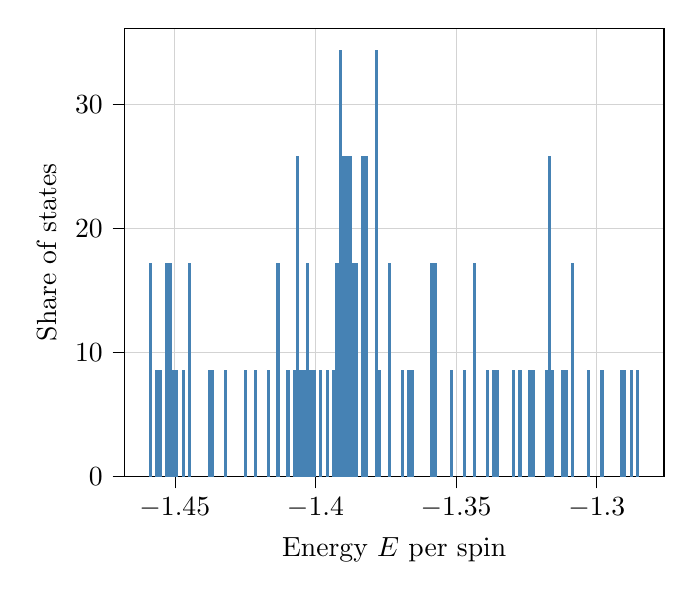
\begin{tikzpicture}

\definecolor{lightgray}{RGB}{211,211,211}
\definecolor{steelblue}{RGB}{70,130,180}

\begin{axis}[
tick align=outside,
tick pos=left,
x grid style={lightgray},
xlabel={Energy \(\displaystyle E\) per spin},
xmajorgrids,
xmin=-1.46792, xmax=-1.27608,
xtick style={color=black},
y grid style={lightgray},
ylabel={Share of states},
ymajorgrids,
ymin=0, ymax=36.1238532110098,
ytick style={color=black}
]
\draw[draw=none,fill=steelblue] (axis cs:-1.4592,0) rectangle (axis cs:-1.45803733333333,17.2018348623856);

\draw[draw=none,fill=steelblue] (axis cs:-1.45803733333333,0) rectangle (axis cs:-1.45687466666667,0);
\draw[draw=none,fill=steelblue] (axis cs:-1.45687466666667,0) rectangle (axis cs:-1.455712,8.60091743119282);
\draw[draw=none,fill=steelblue] (axis cs:-1.455712,0) rectangle (axis cs:-1.45454933333333,8.60091743119282);
\draw[draw=none,fill=steelblue] (axis cs:-1.45454933333333,0) rectangle (axis cs:-1.45338666666667,0);
\draw[draw=none,fill=steelblue] (axis cs:-1.45338666666667,0) rectangle (axis cs:-1.452224,17.2018348623824);
\draw[draw=none,fill=steelblue] (axis cs:-1.452224,0) rectangle (axis cs:-1.45106133333333,17.2018348623856);
\draw[draw=none,fill=steelblue] (axis cs:-1.45106133333333,0) rectangle (axis cs:-1.44989866666667,8.60091743119282);
\draw[draw=none,fill=steelblue] (axis cs:-1.44989866666667,0) rectangle (axis cs:-1.448736,8.60091743119282);
\draw[draw=none,fill=steelblue] (axis cs:-1.448736,0) rectangle (axis cs:-1.44757333333333,0);
\draw[draw=none,fill=steelblue] (axis cs:-1.44757333333333,0) rectangle (axis cs:-1.44641066666667,8.60091743119282);
\draw[draw=none,fill=steelblue] (axis cs:-1.44641066666667,0) rectangle (axis cs:-1.445248,0);
\draw[draw=none,fill=steelblue] (axis cs:-1.445248,0) rectangle (axis cs:-1.44408533333333,17.2018348623856);
\draw[draw=none,fill=steelblue] (axis cs:-1.44408533333333,0) rectangle (axis cs:-1.44292266666667,0);
\draw[draw=none,fill=steelblue] (axis cs:-1.44292266666667,0) rectangle (axis cs:-1.44176,0);
\draw[draw=none,fill=steelblue] (axis cs:-1.44176,0) rectangle (axis cs:-1.44059733333333,0);
\draw[draw=none,fill=steelblue] (axis cs:-1.44059733333333,0) rectangle (axis cs:-1.43943466666667,0);
\draw[draw=none,fill=steelblue] (axis cs:-1.43943466666667,0) rectangle (axis cs:-1.438272,0);
\draw[draw=none,fill=steelblue] (axis cs:-1.438272,0) rectangle (axis cs:-1.43710933333333,8.60091743119282);
\draw[draw=none,fill=steelblue] (axis cs:-1.43710933333333,0) rectangle (axis cs:-1.43594666666667,8.60091743119282);
\draw[draw=none,fill=steelblue] (axis cs:-1.43594666666667,0) rectangle (axis cs:-1.434784,0);
\draw[draw=none,fill=steelblue] (axis cs:-1.434784,0) rectangle (axis cs:-1.43362133333333,0);
\draw[draw=none,fill=steelblue] (axis cs:-1.43362133333333,0) rectangle (axis cs:-1.43245866666667,0);
\draw[draw=none,fill=steelblue] (axis cs:-1.43245866666667,0) rectangle (axis cs:-1.431296,8.60091743119282);
\draw[draw=none,fill=steelblue] (axis cs:-1.431296,0) rectangle (axis cs:-1.43013333333333,0);
\draw[draw=none,fill=steelblue] (axis cs:-1.43013333333333,0) rectangle (axis cs:-1.42897066666667,0);
\draw[draw=none,fill=steelblue] (axis cs:-1.42897066666667,0) rectangle (axis cs:-1.427808,0);
\draw[draw=none,fill=steelblue] (axis cs:-1.427808,0) rectangle (axis cs:-1.42664533333333,0);
\draw[draw=none,fill=steelblue] (axis cs:-1.42664533333333,0) rectangle (axis cs:-1.42548266666667,0);
\draw[draw=none,fill=steelblue] (axis cs:-1.42548266666667,0) rectangle (axis cs:-1.42432,8.60091743119282);
\draw[draw=none,fill=steelblue] (axis cs:-1.42432,0) rectangle (axis cs:-1.42315733333333,0);
\draw[draw=none,fill=steelblue] (axis cs:-1.42315733333333,0) rectangle (axis cs:-1.42199466666667,0);
\draw[draw=none,fill=steelblue] (axis cs:-1.42199466666667,0) rectangle (axis cs:-1.420832,8.60091743119282);
\draw[draw=none,fill=steelblue] (axis cs:-1.420832,0) rectangle (axis cs:-1.41966933333333,0);
\draw[draw=none,fill=steelblue] (axis cs:-1.41966933333333,0) rectangle (axis cs:-1.41850666666667,0);
\draw[draw=none,fill=steelblue] (axis cs:-1.41850666666667,0) rectangle (axis cs:-1.417344,0);
\draw[draw=none,fill=steelblue] (axis cs:-1.417344,0) rectangle (axis cs:-1.41618133333333,8.60091743119282);
\draw[draw=none,fill=steelblue] (axis cs:-1.41618133333333,0) rectangle (axis cs:-1.41501866666667,0);
\draw[draw=none,fill=steelblue] (axis cs:-1.41501866666667,0) rectangle (axis cs:-1.413856,0);
\draw[draw=none,fill=steelblue] (axis cs:-1.413856,0) rectangle (axis cs:-1.41269333333333,17.2018348623856);
\draw[draw=none,fill=steelblue] (axis cs:-1.41269333333333,0) rectangle (axis cs:-1.41153066666667,0);
\draw[draw=none,fill=steelblue] (axis cs:-1.41153066666667,0) rectangle (axis cs:-1.410368,0);
\draw[draw=none,fill=steelblue] (axis cs:-1.410368,0) rectangle (axis cs:-1.40920533333333,8.60091743119282);
\draw[draw=none,fill=steelblue] (axis cs:-1.40920533333333,0) rectangle (axis cs:-1.40804266666667,0);
\draw[draw=none,fill=steelblue] (axis cs:-1.40804266666667,0) rectangle (axis cs:-1.40688,8.60091743119282);
\draw[draw=none,fill=steelblue] (axis cs:-1.40688,0) rectangle (axis cs:-1.40571733333333,25.8027522935735);
\draw[draw=none,fill=steelblue] (axis cs:-1.40571733333333,0) rectangle (axis cs:-1.40455466666667,8.60091743119282);
\draw[draw=none,fill=steelblue] (axis cs:-1.40455466666667,0) rectangle (axis cs:-1.403392,8.60091743119282);
\draw[draw=none,fill=steelblue] (axis cs:-1.403392,0) rectangle (axis cs:-1.40222933333333,17.2018348623856);
\draw[draw=none,fill=steelblue] (axis cs:-1.40222933333333,0) rectangle (axis cs:-1.40106666666667,8.60091743119282);
\draw[draw=none,fill=steelblue] (axis cs:-1.40106666666667,0) rectangle (axis cs:-1.399904,8.60091743119282);
\draw[draw=none,fill=steelblue] (axis cs:-1.399904,0) rectangle (axis cs:-1.39874133333333,0);
\draw[draw=none,fill=steelblue] (axis cs:-1.39874133333333,0) rectangle (axis cs:-1.39757866666667,8.60091743119282);
\draw[draw=none,fill=steelblue] (axis cs:-1.39757866666667,0) rectangle (axis cs:-1.396416,0);
\draw[draw=none,fill=steelblue] (axis cs:-1.396416,0) rectangle (axis cs:-1.39525333333333,8.60091743119118);
\draw[draw=none,fill=steelblue] (axis cs:-1.39525333333333,0) rectangle (axis cs:-1.39409066666667,0);
\draw[draw=none,fill=steelblue] (axis cs:-1.39409066666667,0) rectangle (axis cs:-1.392928,8.60091743119282);
\draw[draw=none,fill=steelblue] (axis cs:-1.392928,0) rectangle (axis cs:-1.39176533333333,17.2018348623856);
\draw[draw=none,fill=steelblue] (axis cs:-1.39176533333333,0) rectangle (axis cs:-1.39060266666667,34.4036697247713);
\draw[draw=none,fill=steelblue] (axis cs:-1.39060266666667,0) rectangle (axis cs:-1.38944,25.8027522935785);
\draw[draw=none,fill=steelblue] (axis cs:-1.38944,0) rectangle (axis cs:-1.38827733333333,25.8027522935785);
\draw[draw=none,fill=steelblue] (axis cs:-1.38827733333333,0) rectangle (axis cs:-1.38711466666667,25.8027522935785);
\draw[draw=none,fill=steelblue] (axis cs:-1.38711466666667,0) rectangle (axis cs:-1.385952,17.2018348623856);
\draw[draw=none,fill=steelblue] (axis cs:-1.385952,0) rectangle (axis cs:-1.38478933333333,17.2018348623856);
\draw[draw=none,fill=steelblue] (axis cs:-1.38478933333333,0) rectangle (axis cs:-1.38362666666667,0);
\draw[draw=none,fill=steelblue] (axis cs:-1.38362666666667,0) rectangle (axis cs:-1.382464,25.8027522935735);
\draw[draw=none,fill=steelblue] (axis cs:-1.382464,0) rectangle (axis cs:-1.38130133333333,25.8027522935785);
\draw[draw=none,fill=steelblue] (axis cs:-1.38130133333333,0) rectangle (axis cs:-1.38013866666667,0);
\draw[draw=none,fill=steelblue] (axis cs:-1.38013866666667,0) rectangle (axis cs:-1.378976,0);
\draw[draw=none,fill=steelblue] (axis cs:-1.378976,0) rectangle (axis cs:-1.37781333333333,34.4036697247713);
\draw[draw=none,fill=steelblue] (axis cs:-1.37781333333333,0) rectangle (axis cs:-1.37665066666667,8.60091743119282);
\draw[draw=none,fill=steelblue] (axis cs:-1.37665066666667,0) rectangle (axis cs:-1.375488,0);
\draw[draw=none,fill=steelblue] (axis cs:-1.375488,0) rectangle (axis cs:-1.37432533333333,0);
\draw[draw=none,fill=steelblue] (axis cs:-1.37432533333333,0) rectangle (axis cs:-1.37316266666667,17.2018348623856);
\draw[draw=none,fill=steelblue] (axis cs:-1.37316266666667,0) rectangle (axis cs:-1.372,0);
\draw[draw=none,fill=steelblue] (axis cs:-1.372,0) rectangle (axis cs:-1.37083733333333,0);
\draw[draw=none,fill=steelblue] (axis cs:-1.37083733333333,0) rectangle (axis cs:-1.36967466666667,0);
\draw[draw=none,fill=steelblue] (axis cs:-1.36967466666667,0) rectangle (axis cs:-1.368512,8.60091743119282);
\draw[draw=none,fill=steelblue] (axis cs:-1.368512,0) rectangle (axis cs:-1.36734933333333,0);
\draw[draw=none,fill=steelblue] (axis cs:-1.36734933333333,0) rectangle (axis cs:-1.36618666666667,8.60091743119282);
\draw[draw=none,fill=steelblue] (axis cs:-1.36618666666667,0) rectangle (axis cs:-1.365024,8.60091743119282);
\draw[draw=none,fill=steelblue] (axis cs:-1.365024,0) rectangle (axis cs:-1.36386133333333,0);
\draw[draw=none,fill=steelblue] (axis cs:-1.36386133333333,0) rectangle (axis cs:-1.36269866666667,0);
\draw[draw=none,fill=steelblue] (axis cs:-1.36269866666667,0) rectangle (axis cs:-1.361536,0);
\draw[draw=none,fill=steelblue] (axis cs:-1.361536,0) rectangle (axis cs:-1.36037333333333,0);
\draw[draw=none,fill=steelblue] (axis cs:-1.36037333333333,0) rectangle (axis cs:-1.35921066666667,0);
\draw[draw=none,fill=steelblue] (axis cs:-1.35921066666667,0) rectangle (axis cs:-1.358048,17.2018348623856);
\draw[draw=none,fill=steelblue] (axis cs:-1.358048,0) rectangle (axis cs:-1.35688533333333,17.2018348623856);
\draw[draw=none,fill=steelblue] (axis cs:-1.35688533333333,0) rectangle (axis cs:-1.35572266666667,0);
\draw[draw=none,fill=steelblue] (axis cs:-1.35572266666667,0) rectangle (axis cs:-1.35456,0);
\draw[draw=none,fill=steelblue] (axis cs:-1.35456,0) rectangle (axis cs:-1.35339733333333,0);
\draw[draw=none,fill=steelblue] (axis cs:-1.35339733333333,0) rectangle (axis cs:-1.35223466666667,0);
\draw[draw=none,fill=steelblue] (axis cs:-1.35223466666667,0) rectangle (axis cs:-1.351072,8.60091743119282);
\draw[draw=none,fill=steelblue] (axis cs:-1.351072,0) rectangle (axis cs:-1.34990933333333,0);
\draw[draw=none,fill=steelblue] (axis cs:-1.34990933333333,0) rectangle (axis cs:-1.34874666666667,0);
\draw[draw=none,fill=steelblue] (axis cs:-1.34874666666667,0) rectangle (axis cs:-1.347584,0);
\draw[draw=none,fill=steelblue] (axis cs:-1.347584,0) rectangle (axis cs:-1.34642133333333,8.60091743119282);
\draw[draw=none,fill=steelblue] (axis cs:-1.34642133333333,0) rectangle (axis cs:-1.34525866666667,0);
\draw[draw=none,fill=steelblue] (axis cs:-1.34525866666667,0) rectangle (axis cs:-1.344096,0);
\draw[draw=none,fill=steelblue] (axis cs:-1.344096,0) rectangle (axis cs:-1.34293333333333,17.2018348623856);
\draw[draw=none,fill=steelblue] (axis cs:-1.34293333333333,0) rectangle (axis cs:-1.34177066666667,0);
\draw[draw=none,fill=steelblue] (axis cs:-1.34177066666667,0) rectangle (axis cs:-1.340608,0);
\draw[draw=none,fill=steelblue] (axis cs:-1.340608,0) rectangle (axis cs:-1.33944533333333,0);
\draw[draw=none,fill=steelblue] (axis cs:-1.33944533333333,0) rectangle (axis cs:-1.33828266666667,8.60091743119282);
\draw[draw=none,fill=steelblue] (axis cs:-1.33828266666667,0) rectangle (axis cs:-1.33712,0);
\draw[draw=none,fill=steelblue] (axis cs:-1.33712,0) rectangle (axis cs:-1.33595733333333,8.60091743119118);
\draw[draw=none,fill=steelblue] (axis cs:-1.33595733333333,0) rectangle (axis cs:-1.33479466666667,8.60091743119282);
\draw[draw=none,fill=steelblue] (axis cs:-1.33479466666667,0) rectangle (axis cs:-1.333632,0);
\draw[draw=none,fill=steelblue] (axis cs:-1.333632,0) rectangle (axis cs:-1.33246933333333,0);
\draw[draw=none,fill=steelblue] (axis cs:-1.33246933333333,0) rectangle (axis cs:-1.33130666666667,0);
\draw[draw=none,fill=steelblue] (axis cs:-1.33130666666667,0) rectangle (axis cs:-1.330144,0);
\draw[draw=none,fill=steelblue] (axis cs:-1.330144,0) rectangle (axis cs:-1.32898133333333,8.60091743119282);
\draw[draw=none,fill=steelblue] (axis cs:-1.32898133333333,0) rectangle (axis cs:-1.32781866666667,0);
\draw[draw=none,fill=steelblue] (axis cs:-1.32781866666667,0) rectangle (axis cs:-1.326656,8.60091743119282);
\draw[draw=none,fill=steelblue] (axis cs:-1.326656,0) rectangle (axis cs:-1.32549333333333,0);
\draw[draw=none,fill=steelblue] (axis cs:-1.32549333333333,0) rectangle (axis cs:-1.32433066666667,0);
\draw[draw=none,fill=steelblue] (axis cs:-1.32433066666667,0) rectangle (axis cs:-1.323168,8.60091743119282);
\draw[draw=none,fill=steelblue] (axis cs:-1.323168,0) rectangle (axis cs:-1.32200533333333,8.60091743119282);
\draw[draw=none,fill=steelblue] (axis cs:-1.32200533333333,0) rectangle (axis cs:-1.32084266666667,0);
\draw[draw=none,fill=steelblue] (axis cs:-1.32084266666667,0) rectangle (axis cs:-1.31968,0);
\draw[draw=none,fill=steelblue] (axis cs:-1.31968,0) rectangle (axis cs:-1.31851733333333,0);
\draw[draw=none,fill=steelblue] (axis cs:-1.31851733333333,0) rectangle (axis cs:-1.31735466666667,8.60091743119282);
\draw[draw=none,fill=steelblue] (axis cs:-1.31735466666667,0) rectangle (axis cs:-1.316192,25.8027522935785);
\draw[draw=none,fill=steelblue] (axis cs:-1.316192,0) rectangle (axis cs:-1.31502933333333,8.60091743119282);
\draw[draw=none,fill=steelblue] (axis cs:-1.31502933333333,0) rectangle (axis cs:-1.31386666666667,0);
\draw[draw=none,fill=steelblue] (axis cs:-1.31386666666667,0) rectangle (axis cs:-1.312704,0);
\draw[draw=none,fill=steelblue] (axis cs:-1.312704,0) rectangle (axis cs:-1.31154133333333,8.60091743119118);
\draw[draw=none,fill=steelblue] (axis cs:-1.31154133333333,0) rectangle (axis cs:-1.31037866666667,8.60091743119282);
\draw[draw=none,fill=steelblue] (axis cs:-1.31037866666667,0) rectangle (axis cs:-1.309216,0);
\draw[draw=none,fill=steelblue] (axis cs:-1.309216,0) rectangle (axis cs:-1.30805333333333,17.2018348623856);
\draw[draw=none,fill=steelblue] (axis cs:-1.30805333333333,0) rectangle (axis cs:-1.30689066666667,0);
\draw[draw=none,fill=steelblue] (axis cs:-1.30689066666667,0) rectangle (axis cs:-1.305728,0);
\draw[draw=none,fill=steelblue] (axis cs:-1.305728,0) rectangle (axis cs:-1.30456533333333,0);
\draw[draw=none,fill=steelblue] (axis cs:-1.30456533333333,0) rectangle (axis cs:-1.30340266666667,0);
\draw[draw=none,fill=steelblue] (axis cs:-1.30340266666667,0) rectangle (axis cs:-1.30224,8.60091743119118);
\draw[draw=none,fill=steelblue] (axis cs:-1.30224,0) rectangle (axis cs:-1.30107733333333,0);
\draw[draw=none,fill=steelblue] (axis cs:-1.30107733333333,0) rectangle (axis cs:-1.29991466666667,0);
\draw[draw=none,fill=steelblue] (axis cs:-1.29991466666667,0) rectangle (axis cs:-1.298752,0);
\draw[draw=none,fill=steelblue] (axis cs:-1.298752,0) rectangle (axis cs:-1.29758933333333,8.60091743119282);
\draw[draw=none,fill=steelblue] (axis cs:-1.29758933333333,0) rectangle (axis cs:-1.29642666666667,0);
\draw[draw=none,fill=steelblue] (axis cs:-1.29642666666667,0) rectangle (axis cs:-1.295264,0);
\draw[draw=none,fill=steelblue] (axis cs:-1.295264,0) rectangle (axis cs:-1.29410133333333,0);
\draw[draw=none,fill=steelblue] (axis cs:-1.29410133333333,0) rectangle (axis cs:-1.29293866666667,0);
\draw[draw=none,fill=steelblue] (axis cs:-1.29293866666667,0) rectangle (axis cs:-1.291776,0);
\draw[draw=none,fill=steelblue] (axis cs:-1.291776,0) rectangle (axis cs:-1.29061333333333,8.60091743119282);
\draw[draw=none,fill=steelblue] (axis cs:-1.29061333333333,0) rectangle (axis cs:-1.28945066666667,8.60091743119282);
\draw[draw=none,fill=steelblue] (axis cs:-1.28945066666667,0) rectangle (axis cs:-1.288288,0);
\draw[draw=none,fill=steelblue] (axis cs:-1.288288,0) rectangle (axis cs:-1.28712533333333,8.60091743119282);
\draw[draw=none,fill=steelblue] (axis cs:-1.28712533333333,0) rectangle (axis cs:-1.28596266666667,0);
\draw[draw=none,fill=steelblue] (axis cs:-1.28596266666667,0) rectangle (axis cs:-1.2848,8.60091743119282);
\end{axis}

\end{tikzpicture}

\end{figure}

\begin{figure}
\centering
% This file was created with tikzplotlib v0.10.1.
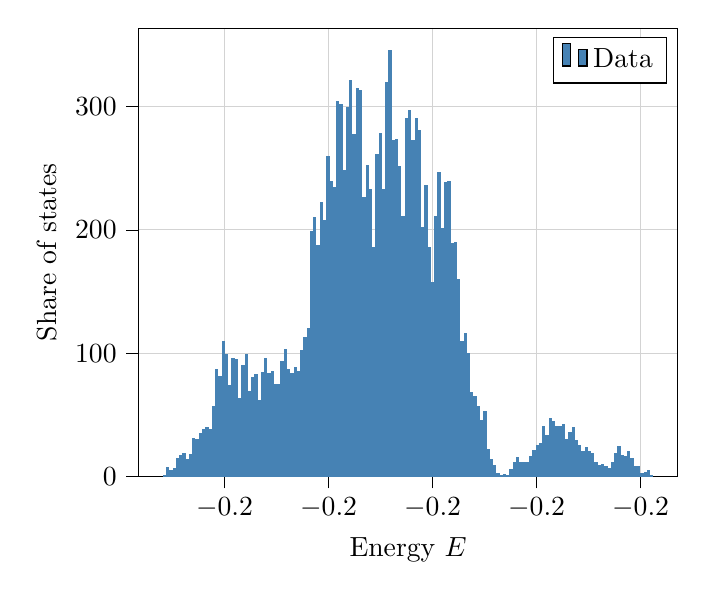
\begin{tikzpicture}

\definecolor{lightgray}{RGB}{211,211,211}
\definecolor{steelblue}{RGB}{70,130,180}

\begin{axis}[
tick align=outside,
tick pos=left,
x grid style={lightgray},
xlabel={Energy \(\displaystyle E\)},
xmajorgrids,
xmin=-0.205660555555556, xmax=-0.195283888888889,
xtick style={color=black},
y grid style={lightgray},
ylabel={Share of states},
ymajorgrids,
ymin=0, ymax=363.440989399286,
ytick style={color=black}
]
\draw[draw=none,fill=steelblue] (axis cs:-0.205188888888889,0) rectangle (axis cs:-0.205126,1.08127208480563);
\addlegendimage{ybar,ybar legend,draw=none,fill=steelblue}
\addlegendentry{Data}

\draw[draw=none,fill=steelblue] (axis cs:-0.205126,0) rectangle (axis cs:-0.205063111111111,7.4734982332154);
\draw[draw=none,fill=steelblue] (axis cs:-0.205063111111111,0) rectangle (axis cs:-0.205000222222222,5.15194346289743);
\draw[draw=none,fill=steelblue] (axis cs:-0.205000222222222,0) rectangle (axis cs:-0.204937333333333,6.55123674911648);
\draw[draw=none,fill=steelblue] (axis cs:-0.204937333333333,0) rectangle (axis cs:-0.204874444444444,15.2650176678442);
\draw[draw=none,fill=steelblue] (axis cs:-0.204874444444444,0) rectangle (axis cs:-0.204811555555556,17.5865724381622);
\draw[draw=none,fill=steelblue] (axis cs:-0.204811555555556,0) rectangle (axis cs:-0.204748666666667,19.1130742049466);
\draw[draw=none,fill=steelblue] (axis cs:-0.204748666666667,0) rectangle (axis cs:-0.204685777777778,13.8339222614838);
\draw[draw=none,fill=steelblue] (axis cs:-0.204685777777778,0) rectangle (axis cs:-0.204622888888889,18.5724381625438);
\draw[draw=none,fill=steelblue] (axis cs:-0.204622888888889,0) rectangle (axis cs:-0.20456,31.3886925795047);
\draw[draw=none,fill=steelblue] (axis cs:-0.20456,0) rectangle (axis cs:-0.204497111111111,30.0848056537097);
\draw[draw=none,fill=steelblue] (axis cs:-0.204497111111111,0) rectangle (axis cs:-0.204434222222222,35.5865724381619);
\draw[draw=none,fill=steelblue] (axis cs:-0.204434222222222,0) rectangle (axis cs:-0.204371333333333,38.92579505302);
\draw[draw=none,fill=steelblue] (axis cs:-0.204371333333333,0) rectangle (axis cs:-0.204308444444444,39.9434628975257);
\draw[draw=none,fill=steelblue] (axis cs:-0.204308444444444,0) rectangle (axis cs:-0.204245555555556,38.2261484098932);
\draw[draw=none,fill=steelblue] (axis cs:-0.204245555555556,0) rectangle (axis cs:-0.204182666666667,57.4982332155466);
\draw[draw=none,fill=steelblue] (axis cs:-0.204182666666667,0) rectangle (axis cs:-0.204119777777778,86.9787985865708);
\draw[draw=none,fill=steelblue] (axis cs:-0.204119777777778,0) rectangle (axis cs:-0.204056888888889,81.2544169611292);
\draw[draw=none,fill=steelblue] (axis cs:-0.204056888888889,0) rectangle (axis cs:-0.203994,109.558303886924);
\draw[draw=none,fill=steelblue] (axis cs:-0.203994,0) rectangle (axis cs:-0.203931111111111,98.9681978798567);
\draw[draw=none,fill=steelblue] (axis cs:-0.203931111111111,0) rectangle (axis cs:-0.203868222222222,74.5759717314473);
\draw[draw=none,fill=steelblue] (axis cs:-0.203868222222222,0) rectangle (axis cs:-0.203805333333333,96.1696113074186);
\draw[draw=none,fill=steelblue] (axis cs:-0.203805333333333,0) rectangle (axis cs:-0.203742444444444,95.6925795052985);
\draw[draw=none,fill=steelblue] (axis cs:-0.203742444444444,0) rectangle (axis cs:-0.203679555555556,63.954063604239);
\draw[draw=none,fill=steelblue] (axis cs:-0.203679555555556,0) rectangle (axis cs:-0.203616666666667,90.5724381625424);
\draw[draw=none,fill=steelblue] (axis cs:-0.203616666666667,0) rectangle (axis cs:-0.203553777777778,99.1908127208461);
\draw[draw=none,fill=steelblue] (axis cs:-0.203553777777778,0) rectangle (axis cs:-0.203490888888889,69.3604240282672);
\draw[draw=none,fill=steelblue] (axis cs:-0.203490888888889,0) rectangle (axis cs:-0.203428,80.7455830388677);
\draw[draw=none,fill=steelblue] (axis cs:-0.203428,0) rectangle (axis cs:-0.203365111111111,83.1625441696097);
\draw[draw=none,fill=steelblue] (axis cs:-0.203365111111111,0) rectangle (axis cs:-0.203302222222222,61.8551236749105);
\draw[draw=none,fill=steelblue] (axis cs:-0.203302222222222,0) rectangle (axis cs:-0.203239333333333,84.402826855122);
\draw[draw=none,fill=steelblue] (axis cs:-0.203239333333333,0) rectangle (axis cs:-0.203176444444444,95.9787985865706);
\draw[draw=none,fill=steelblue] (axis cs:-0.203176444444444,0) rectangle (axis cs:-0.203113555555556,84.212014134274);
\draw[draw=none,fill=steelblue] (axis cs:-0.203113555555556,0) rectangle (axis cs:-0.203050666666667,85.611307420493);
\draw[draw=none,fill=steelblue] (axis cs:-0.203050666666667,0) rectangle (axis cs:-0.202987777777778,75.1484098939915);
\draw[draw=none,fill=steelblue] (axis cs:-0.202987777777778,0) rectangle (axis cs:-0.202924888888889,75.0530035335675);
\draw[draw=none,fill=steelblue] (axis cs:-0.202924888888889,0) rectangle (axis cs:-0.202862,93.4028268551219);
\draw[draw=none,fill=steelblue] (axis cs:-0.202862,0) rectangle (axis cs:-0.202799111111111,103.42049469969);
\draw[draw=none,fill=steelblue] (axis cs:-0.202799111111111,0) rectangle (axis cs:-0.202736222222222,87.5194346289736);
\draw[draw=none,fill=steelblue] (axis cs:-0.202736222222222,0) rectangle (axis cs:-0.202673333333333,83.9257950530019);
\draw[draw=none,fill=steelblue] (axis cs:-0.202673333333333,0) rectangle (axis cs:-0.202610444444444,89.141342756182);
\draw[draw=none,fill=steelblue] (axis cs:-0.202610444444444,0) rectangle (axis cs:-0.202547555555556,85.3568904593623);
\draw[draw=none,fill=steelblue] (axis cs:-0.202547555555556,0) rectangle (axis cs:-0.202484666666667,102.339222614839);
\draw[draw=none,fill=steelblue] (axis cs:-0.202484666666667,0) rectangle (axis cs:-0.202421777777778,113.374558303885);
\draw[draw=none,fill=steelblue] (axis cs:-0.202421777777778,0) rectangle (axis cs:-0.202358888888889,120.561837455828);
\draw[draw=none,fill=steelblue] (axis cs:-0.202358888888889,0) rectangle (axis cs:-0.202296,199.399293286215);
\draw[draw=none,fill=steelblue] (axis cs:-0.202296,0) rectangle (axis cs:-0.202233111111111,210.65724381625);
\draw[draw=none,fill=steelblue] (axis cs:-0.202233111111111,0) rectangle (axis cs:-0.202170222222222,187.314487632505);
\draw[draw=none,fill=steelblue] (axis cs:-0.202170222222222,0) rectangle (axis cs:-0.202107333333333,222.169611307416);
\draw[draw=none,fill=steelblue] (axis cs:-0.202107333333333,0) rectangle (axis cs:-0.202044444444444,208.367491166074);
\draw[draw=none,fill=steelblue] (axis cs:-0.202044444444444,0) rectangle (axis cs:-0.201981555555556,259.6961130742);
\draw[draw=none,fill=steelblue] (axis cs:-0.201981555555556,0) rectangle (axis cs:-0.201918666666667,239.819787985861);
\draw[draw=none,fill=steelblue] (axis cs:-0.201918666666667,0) rectangle (axis cs:-0.201855777777778,234.763250883388);
\draw[draw=none,fill=steelblue] (axis cs:-0.201855777777778,0) rectangle (axis cs:-0.201792888888889,304.568904593634);
\draw[draw=none,fill=steelblue] (axis cs:-0.201792888888889,0) rectangle (axis cs:-0.20173,302.056537102468);
\draw[draw=none,fill=steelblue] (axis cs:-0.20173,0) rectangle (axis cs:-0.201667111111111,248.533568904589);
\draw[draw=none,fill=steelblue] (axis cs:-0.201667111111111,0) rectangle (axis cs:-0.201604222222222,299.25795053003);
\draw[draw=none,fill=steelblue] (axis cs:-0.201604222222222,0) rectangle (axis cs:-0.201541333333333,321.742049469958);
\draw[draw=none,fill=steelblue] (axis cs:-0.201541333333333,0) rectangle (axis cs:-0.201478444444444,277.855123674906);
\draw[draw=none,fill=steelblue] (axis cs:-0.201478444444444,0) rectangle (axis cs:-0.201415555555556,314.745583038863);
\draw[draw=none,fill=steelblue] (axis cs:-0.201415555555556,0) rectangle (axis cs:-0.201352666666667,312.964664310948);
\draw[draw=none,fill=steelblue] (axis cs:-0.201352666666667,0) rectangle (axis cs:-0.201289777777778,226.685512367487);
\draw[draw=none,fill=steelblue] (axis cs:-0.201289777777778,0) rectangle (axis cs:-0.201226888888889,252.540636042509);
\draw[draw=none,fill=steelblue] (axis cs:-0.201226888888889,0) rectangle (axis cs:-0.201164,233.39575971731);
\draw[draw=none,fill=steelblue] (axis cs:-0.201164,0) rectangle (axis cs:-0.201101111111111,185.787985865721);
\draw[draw=none,fill=steelblue] (axis cs:-0.201101111111111,0) rectangle (axis cs:-0.201038222222222,261.222614840984);
\draw[draw=none,fill=steelblue] (axis cs:-0.201038222222222,0) rectangle (axis cs:-0.200975333333333,278.491166077733);
\draw[draw=none,fill=steelblue] (axis cs:-0.200975333333333,0) rectangle (axis cs:-0.200912444444444,232.727915194342);
\draw[draw=none,fill=steelblue] (axis cs:-0.200912444444444,0) rectangle (axis cs:-0.200849555555556,319.865724381619);
\draw[draw=none,fill=steelblue] (axis cs:-0.200849555555556,0) rectangle (axis cs:-0.200786666666667,346.134275618368);
\draw[draw=none,fill=steelblue] (axis cs:-0.200786666666667,0) rectangle (axis cs:-0.200723777777778,273.021201413422);
\draw[draw=none,fill=steelblue] (axis cs:-0.200723777777778,0) rectangle (axis cs:-0.200660888888889,273.91166077738);
\draw[draw=none,fill=steelblue] (axis cs:-0.200660888888889,0) rectangle (axis cs:-0.200598,251.522968197875);
\draw[draw=none,fill=steelblue] (axis cs:-0.200598,0) rectangle (axis cs:-0.200535111111111,211.35689045936);
\draw[draw=none,fill=steelblue] (axis cs:-0.200535111111111,0) rectangle (axis cs:-0.200472222222222,290.448763250878);
\draw[draw=none,fill=steelblue] (axis cs:-0.200472222222222,0) rectangle (axis cs:-0.200409333333333,297.477031802114);
\draw[draw=none,fill=steelblue] (axis cs:-0.200409333333333,0) rectangle (axis cs:-0.200346444444444,272.989399293281);
\draw[draw=none,fill=steelblue] (axis cs:-0.200346444444444,0) rectangle (axis cs:-0.200283555555556,291.053003533563);
\draw[draw=none,fill=steelblue] (axis cs:-0.200283555555556,0) rectangle (axis cs:-0.200220666666667,280.717314487627);
\draw[draw=none,fill=steelblue] (axis cs:-0.200220666666667,0) rectangle (axis cs:-0.200157777777778,202.197879858653);
\draw[draw=none,fill=steelblue] (axis cs:-0.200157777777778,0) rectangle (axis cs:-0.200094888888889,236.321554770313);
\draw[draw=none,fill=steelblue] (axis cs:-0.200094888888889,0) rectangle (axis cs:-0.200032,186.455830388689);
\draw[draw=none,fill=steelblue] (axis cs:-0.200032,0) rectangle (axis cs:-0.199969111111111,157.420494699644);
\draw[draw=none,fill=steelblue] (axis cs:-0.199969111111111,0) rectangle (axis cs:-0.199906222222222,211.484098939925);
\draw[draw=none,fill=steelblue] (axis cs:-0.199906222222222,0) rectangle (axis cs:-0.199843333333333,246.530035335684);
\draw[draw=none,fill=steelblue] (axis cs:-0.199843333333333,0) rectangle (axis cs:-0.199780444444444,201.148409893989);
\draw[draw=none,fill=steelblue] (axis cs:-0.199780444444444,0) rectangle (axis cs:-0.199717555555556,238.643109540631);
\draw[draw=none,fill=steelblue] (axis cs:-0.199717555555556,0) rectangle (axis cs:-0.199654666666667,239.279151943564);
\draw[draw=none,fill=steelblue] (axis cs:-0.199654666666667,0) rectangle (axis cs:-0.199591777777778,189.636042402823);
\draw[draw=none,fill=steelblue] (axis cs:-0.199591777777778,0) rectangle (axis cs:-0.199528888888889,189.79505300353);
\draw[draw=none,fill=steelblue] (axis cs:-0.199528888888889,0) rectangle (axis cs:-0.199466,160.314487632506);
\draw[draw=none,fill=steelblue] (axis cs:-0.199466,0) rectangle (axis cs:-0.199403111111111,109.876325088337);
\draw[draw=none,fill=steelblue] (axis cs:-0.199403111111111,0) rectangle (axis cs:-0.199340222222222,116.554770318019);
\draw[draw=none,fill=steelblue] (axis cs:-0.199340222222222,0) rectangle (axis cs:-0.199277333333333,99.826855123673);
\draw[draw=none,fill=steelblue] (axis cs:-0.199277333333333,0) rectangle (axis cs:-0.199214444444444,68.7561837455817);
\draw[draw=none,fill=steelblue] (axis cs:-0.199214444444444,0) rectangle (axis cs:-0.199151555555556,64.9399293286207);
\draw[draw=none,fill=steelblue] (axis cs:-0.199151555555556,0) rectangle (axis cs:-0.199088666666667,56.8303886925784);
\draw[draw=none,fill=steelblue] (axis cs:-0.199088666666667,0) rectangle (axis cs:-0.199025777777778,45.9222614840981);
\draw[draw=none,fill=steelblue] (axis cs:-0.199025777777778,0) rectangle (axis cs:-0.198962888888889,52.9505300353347);
\draw[draw=none,fill=steelblue] (axis cs:-0.198962888888889,0) rectangle (axis cs:-0.1989,22.6113074204943);
\draw[draw=none,fill=steelblue] (axis cs:-0.1989,0) rectangle (axis cs:-0.198837111111111,13.8975265017665);
\draw[draw=none,fill=steelblue] (axis cs:-0.198837111111111,0) rectangle (axis cs:-0.198774222222222,9.60424028268533);
\draw[draw=none,fill=steelblue] (axis cs:-0.198774222222222,0) rectangle (axis cs:-0.198711333333333,2.51236749116603);
\draw[draw=none,fill=steelblue] (axis cs:-0.198711333333333,0) rectangle (axis cs:-0.198648444444444,0.922261484098922);
\draw[draw=none,fill=steelblue] (axis cs:-0.198648444444444,0) rectangle (axis cs:-0.198585555555556,2.44876325088335);
\draw[draw=none,fill=steelblue] (axis cs:-0.198585555555556,0) rectangle (axis cs:-0.198522666666667,1.33568904593637);
\draw[draw=none,fill=steelblue] (axis cs:-0.198522666666667,0) rectangle (axis cs:-0.198459777777778,6.4876325088338);
\draw[draw=none,fill=steelblue] (axis cs:-0.198459777777778,0) rectangle (axis cs:-0.198396888888889,11.6395759717312);
\draw[draw=none,fill=steelblue] (axis cs:-0.198396888888889,0) rectangle (axis cs:-0.198334,15.519434628975);
\draw[draw=none,fill=steelblue] (axis cs:-0.198334,0) rectangle (axis cs:-0.198271111111111,12.180212014134);
\draw[draw=none,fill=steelblue] (axis cs:-0.198271111111111,0) rectangle (axis cs:-0.198208222222222,11.9257950530033);
\draw[draw=none,fill=steelblue] (axis cs:-0.198208222222222,0) rectangle (axis cs:-0.198145333333333,11.607773851595);
\draw[draw=none,fill=steelblue] (axis cs:-0.198145333333333,0) rectangle (axis cs:-0.198082444444444,17.0459363957594);
\draw[draw=none,fill=steelblue] (axis cs:-0.198082444444444,0) rectangle (axis cs:-0.198019555555556,21.8162544169607);
\draw[draw=none,fill=steelblue] (axis cs:-0.198019555555556,0) rectangle (axis cs:-0.197956666666667,25.5371024734977);
\draw[draw=none,fill=steelblue] (axis cs:-0.197956666666667,0) rectangle (axis cs:-0.197893777777778,27.508833922261);
\draw[draw=none,fill=steelblue] (axis cs:-0.197893777777778,0) rectangle (axis cs:-0.197830888888889,41.2155477031794);
\draw[draw=none,fill=steelblue] (axis cs:-0.197830888888889,0) rectangle (axis cs:-0.197768,34.0600706713774);
\draw[draw=none,fill=steelblue] (axis cs:-0.197768,0) rectangle (axis cs:-0.197705111111111,47.1625441696104);
\draw[draw=none,fill=steelblue] (axis cs:-0.197705111111111,0) rectangle (axis cs:-0.197642222222222,45.3816254416952);
\draw[draw=none,fill=steelblue] (axis cs:-0.197642222222222,0) rectangle (axis cs:-0.197579333333333,40.7067137809179);
\draw[draw=none,fill=steelblue] (axis cs:-0.197579333333333,0) rectangle (axis cs:-0.197516444444444,41.0247349823314);
\draw[draw=none,fill=steelblue] (axis cs:-0.197516444444444,0) rectangle (axis cs:-0.197453555555556,42.4240282685504);
\draw[draw=none,fill=steelblue] (axis cs:-0.197453555555556,0) rectangle (axis cs:-0.197390666666667,30.0848056537097);
\draw[draw=none,fill=steelblue] (axis cs:-0.197390666666667,0) rectangle (axis cs:-0.197327777777778,35.8091872791513);
\draw[draw=none,fill=steelblue] (axis cs:-0.197327777777778,0) rectangle (axis cs:-0.197264888888889,40.4522968197872);
\draw[draw=none,fill=steelblue] (axis cs:-0.197264888888889,0) rectangle (axis cs:-0.197202,29.6713780918722);
\draw[draw=none,fill=steelblue] (axis cs:-0.197202,0) rectangle (axis cs:-0.197139111111111,25.7915194346285);
\draw[draw=none,fill=steelblue] (axis cs:-0.197139111111111,0) rectangle (axis cs:-0.197076222222222,20.353356890459);
\draw[draw=none,fill=steelblue] (axis cs:-0.197076222222222,0) rectangle (axis cs:-0.197013333333333,24.074204946996);
\draw[draw=none,fill=steelblue] (axis cs:-0.197013333333333,0) rectangle (axis cs:-0.196950444444444,20.9893992932858);
\draw[draw=none,fill=steelblue] (axis cs:-0.196950444444444,0) rectangle (axis cs:-0.196887555555556,18.8586572438159);
\draw[draw=none,fill=steelblue] (axis cs:-0.196887555555556,0) rectangle (axis cs:-0.196824666666667,11.8621908127206);
\draw[draw=none,fill=steelblue] (axis cs:-0.196824666666667,0) rectangle (axis cs:-0.196761777777778,9.15901060070654);
\draw[draw=none,fill=steelblue] (axis cs:-0.196761777777778,0) rectangle (axis cs:-0.196698888888889,10.1766784452295);
\draw[draw=none,fill=steelblue] (axis cs:-0.196698888888889,0) rectangle (axis cs:-0.196636,8.36395759717298);
\draw[draw=none,fill=steelblue] (axis cs:-0.196636,0) rectangle (axis cs:-0.196573111111111,7.12367491166064);
\draw[draw=none,fill=steelblue] (axis cs:-0.196573111111111,0) rectangle (axis cs:-0.196510222222222,11.5441696113072);
\draw[draw=none,fill=steelblue] (axis cs:-0.196510222222222,0) rectangle (axis cs:-0.196447333333333,19.2084805653791);
\draw[draw=none,fill=steelblue] (axis cs:-0.196447333333333,0) rectangle (axis cs:-0.196384444444444,24.7738515901055);
\draw[draw=none,fill=steelblue] (axis cs:-0.196384444444444,0) rectangle (axis cs:-0.196321555555556,17.3003533568901);
\draw[draw=none,fill=steelblue] (axis cs:-0.196321555555556,0) rectangle (axis cs:-0.196258666666667,16.82332155477);
\draw[draw=none,fill=steelblue] (axis cs:-0.196258666666667,0) rectangle (axis cs:-0.196195777777778,20.7667844522964);
\draw[draw=none,fill=steelblue] (axis cs:-0.196195777777778,0) rectangle (axis cs:-0.196132888888889,15.0742049469962);
\draw[draw=none,fill=steelblue] (axis cs:-0.196132888888889,0) rectangle (axis cs:-0.19607,8.36395759717298);
\draw[draw=none,fill=steelblue] (axis cs:-0.19607,0) rectangle (axis cs:-0.196007111111111,8.87279151943446);
\draw[draw=none,fill=steelblue] (axis cs:-0.196007111111111,0) rectangle (axis cs:-0.195944222222222,2.76678445229677);
\draw[draw=none,fill=steelblue] (axis cs:-0.195944222222222,0) rectangle (axis cs:-0.195881333333333,3.72084805653703);
\draw[draw=none,fill=steelblue] (axis cs:-0.195881333333333,0) rectangle (axis cs:-0.195818444444444,5.2791519434628);
\draw[draw=none,fill=steelblue] (axis cs:-0.195818444444444,0) rectangle (axis cs:-0.195755555555556,1.30388692579503);
\end{axis}

\end{tikzpicture}

\end{figure}

\begin{figure}
\centering
% This file was created with tikzplotlib v0.10.1.
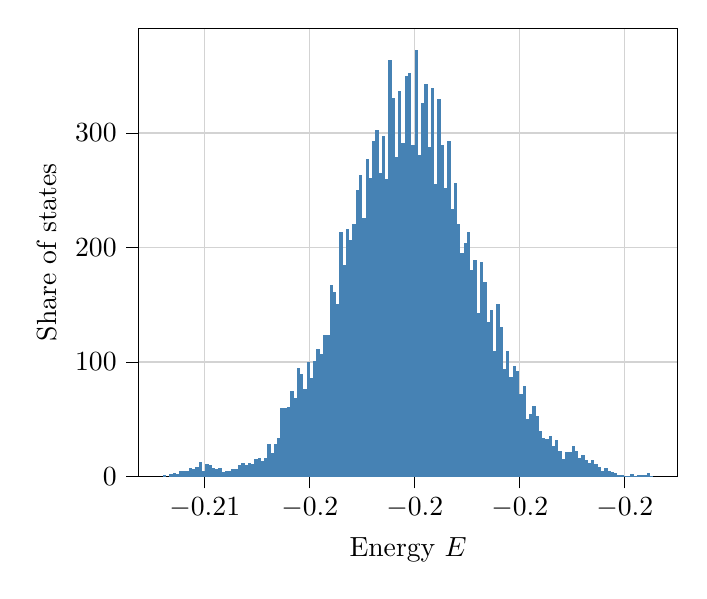
\begin{tikzpicture}

\definecolor{lightgray}{RGB}{211,211,211}
\definecolor{steelblue}{RGB}{70,130,180}

\begin{axis}[
tick align=outside,
tick pos=left,
x grid style={lightgray},
xlabel={Energy \(\displaystyle E\)},
xmajorgrids,
xmin=-0.207267222222222, xmax=-0.196988333333333,
xtick style={color=black},
y grid style={lightgray},
ylabel={Share of states},
ymajorgrids,
ymin=0, ymax=391.539739257018,
ytick style={color=black}
]
\draw[draw=none,fill=steelblue] (axis cs:-0.2068,0) rectangle (axis cs:-0.206737703703704,1.62128256421053);

\draw[draw=none,fill=steelblue] (axis cs:-0.206737703703704,0) rectangle (axis cs:-0.206675407407407,0);
\draw[draw=none,fill=steelblue] (axis cs:-0.206675407407407,0) rectangle (axis cs:-0.206613111111111,2.02660320526407);
\draw[draw=none,fill=steelblue] (axis cs:-0.206613111111111,0) rectangle (axis cs:-0.206550814814815,2.83724448736843);
\draw[draw=none,fill=steelblue] (axis cs:-0.206550814814815,0) rectangle (axis cs:-0.206488518518518,2.4319238463158);
\draw[draw=none,fill=steelblue] (axis cs:-0.206488518518519,0) rectangle (axis cs:-0.206426222222222,4.45852705158095);
\draw[draw=none,fill=steelblue] (axis cs:-0.206426222222222,0) rectangle (axis cs:-0.206363925925926,5.26916833368658);
\draw[draw=none,fill=steelblue] (axis cs:-0.206363925925926,0) rectangle (axis cs:-0.20630162962963,4.45852705157896);
\draw[draw=none,fill=steelblue] (axis cs:-0.20630162962963,0) rectangle (axis cs:-0.206239333333333,7.29577153894739);
\draw[draw=none,fill=steelblue] (axis cs:-0.206239333333333,0) rectangle (axis cs:-0.206177037037037,6.89045089789783);
\draw[draw=none,fill=steelblue] (axis cs:-0.206177037037037,0) rectangle (axis cs:-0.206114740740741,8.10641282105627);
\draw[draw=none,fill=steelblue] (axis cs:-0.206114740740741,0) rectangle (axis cs:-0.206052444444444,12.9702605136843);
\draw[draw=none,fill=steelblue] (axis cs:-0.206052444444444,0) rectangle (axis cs:-0.205990148148148,5.26916833368423);
\draw[draw=none,fill=steelblue] (axis cs:-0.205990148148148,0) rectangle (axis cs:-0.205927851851852,10.5383366673732);
\draw[draw=none,fill=steelblue] (axis cs:-0.205927851851852,0) rectangle (axis cs:-0.205865555555556,9.72769538526753);
\draw[draw=none,fill=steelblue] (axis cs:-0.205865555555556,0) rectangle (axis cs:-0.205803259259259,7.70109218000003);
\draw[draw=none,fill=steelblue] (axis cs:-0.205803259259259,0) rectangle (axis cs:-0.205740962962963,6.48513025684213);
\draw[draw=none,fill=steelblue] (axis cs:-0.205740962962963,0) rectangle (axis cs:-0.205678666666667,7.70109218000346);
\draw[draw=none,fill=steelblue] (axis cs:-0.205678666666667,0) rectangle (axis cs:-0.20561637037037,3.64788576947532);
\draw[draw=none,fill=steelblue] (axis cs:-0.20561637037037,0) rectangle (axis cs:-0.205554074074074,4.45852705157896);
\draw[draw=none,fill=steelblue] (axis cs:-0.205554074074074,0) rectangle (axis cs:-0.205491777777778,4.45852705157896);
\draw[draw=none,fill=steelblue] (axis cs:-0.205491777777778,0) rectangle (axis cs:-0.205429481481481,6.48513025684502);
\draw[draw=none,fill=steelblue] (axis cs:-0.205429481481481,0) rectangle (axis cs:-0.205367185185185,6.48513025684502);
\draw[draw=none,fill=steelblue] (axis cs:-0.205367185185185,0) rectangle (axis cs:-0.205304888888889,10.1330160263158);
\draw[draw=none,fill=steelblue] (axis cs:-0.205304888888889,0) rectangle (axis cs:-0.205242592592593,12.159619231579);
\draw[draw=none,fill=steelblue] (axis cs:-0.205242592592593,0) rectangle (axis cs:-0.205180296296296,9.72769538526753);
\draw[draw=none,fill=steelblue] (axis cs:-0.205180296296296,0) rectangle (axis cs:-0.205118,12.1596192315844);
\draw[draw=none,fill=steelblue] (axis cs:-0.205118,0) rectangle (axis cs:-0.205055703703704,10.9436573084211);
\draw[draw=none,fill=steelblue] (axis cs:-0.205055703703704,0) rectangle (axis cs:-0.204993407407407,15.4021843600001);
\draw[draw=none,fill=steelblue] (axis cs:-0.204993407407407,0) rectangle (axis cs:-0.204931111111111,16.6181462831654);
\draw[draw=none,fill=steelblue] (axis cs:-0.204931111111111,0) rectangle (axis cs:-0.204868814814815,13.7809017957957);
\draw[draw=none,fill=steelblue] (axis cs:-0.204868814814815,0) rectangle (axis cs:-0.204806518518519,16.2128256421053);
\draw[draw=none,fill=steelblue] (axis cs:-0.204806518518518,0) rectangle (axis cs:-0.204744222222222,28.7777655147369);
\draw[draw=none,fill=steelblue] (axis cs:-0.204744222222222,0) rectangle (axis cs:-0.204681925925926,20.2660320526407);
\draw[draw=none,fill=steelblue] (axis cs:-0.204681925925926,0) rectangle (axis cs:-0.20461962962963,28.7777655147498);
\draw[draw=none,fill=steelblue] (axis cs:-0.20461962962963,0) rectangle (axis cs:-0.204557333333333,33.2362925663159);
\draw[draw=none,fill=steelblue] (axis cs:-0.204557333333333,0) rectangle (axis cs:-0.204495037037037,59.582134234737);
\draw[draw=none,fill=steelblue] (axis cs:-0.204495037037037,0) rectangle (axis cs:-0.204432740740741,59.9874548758164);
\draw[draw=none,fill=steelblue] (axis cs:-0.204432740740741,0) rectangle (axis cs:-0.204370444444444,60.3927755168692);
\draw[draw=none,fill=steelblue] (axis cs:-0.204370444444444,0) rectangle (axis cs:-0.204308148148148,74.5789979536845);
\draw[draw=none,fill=steelblue] (axis cs:-0.204308148148148,0) rectangle (axis cs:-0.204245851851852,68.9045089789476);
\draw[draw=none,fill=steelblue] (axis cs:-0.204245851851852,0) rectangle (axis cs:-0.204183555555556,94.8450300063584);
\draw[draw=none,fill=steelblue] (axis cs:-0.204183555555556,0) rectangle (axis cs:-0.204121259259259,89.170541031619);
\draw[draw=none,fill=steelblue] (axis cs:-0.204121259259259,0) rectangle (axis cs:-0.204058962962963,76.200280517895);
\draw[draw=none,fill=steelblue] (axis cs:-0.204058962962963,0) rectangle (axis cs:-0.203996666666667,99.7088776989477);
\draw[draw=none,fill=steelblue] (axis cs:-0.203996666666667,0) rectangle (axis cs:-0.20393437037037,85.9279759031965);
\draw[draw=none,fill=steelblue] (axis cs:-0.20393437037037,0) rectangle (axis cs:-0.203872074074074,100.519518981098);
\draw[draw=none,fill=steelblue] (axis cs:-0.203872074074074,0) rectangle (axis cs:-0.203809777777778,111.463176289474);
\draw[draw=none,fill=steelblue] (axis cs:-0.203809777777778,0) rectangle (axis cs:-0.203747481481481,107.409969878948);
\draw[draw=none,fill=steelblue] (axis cs:-0.203747481481481,0) rectangle (axis cs:-0.203685185185185,124.028116162161);
\draw[draw=none,fill=steelblue] (axis cs:-0.203685185185185,0) rectangle (axis cs:-0.203622888888889,124.028116162161);
\draw[draw=none,fill=steelblue] (axis cs:-0.203622888888889,0) rectangle (axis cs:-0.203560592592593,167.397424754737);
\draw[draw=none,fill=steelblue] (axis cs:-0.203560592592593,0) rectangle (axis cs:-0.203498296296296,161.317615138948);
\draw[draw=none,fill=steelblue] (axis cs:-0.203498296296296,0) rectangle (axis cs:-0.203436,150.373957830594);
\draw[draw=none,fill=steelblue] (axis cs:-0.203436,0) rectangle (axis cs:-0.203373703703704,213.19865719378);
\draw[draw=none,fill=steelblue] (axis cs:-0.203373703703704,0) rectangle (axis cs:-0.203311407407407,184.420891678948);
\draw[draw=none,fill=steelblue] (axis cs:-0.203311407407407,0) rectangle (axis cs:-0.203249111111111,216.441222322106);
\draw[draw=none,fill=steelblue] (axis cs:-0.203249111111111,0) rectangle (axis cs:-0.203186814814815,206.713526936935);
\draw[draw=none,fill=steelblue] (axis cs:-0.203186814814815,0) rectangle (axis cs:-0.203124518518519,220.494428732731);
\draw[draw=none,fill=steelblue] (axis cs:-0.203124518518519,0) rectangle (axis cs:-0.203062222222222,250.488156170527);
\draw[draw=none,fill=steelblue] (axis cs:-0.203062222222222,0) rectangle (axis cs:-0.202999925925926,263.053096043159);
\draw[draw=none,fill=steelblue] (axis cs:-0.202999925925926,0) rectangle (axis cs:-0.20293762962963,225.763597066417);
\draw[draw=none,fill=steelblue] (axis cs:-0.20293762962963,0) rectangle (axis cs:-0.202875333333333,277.239318480124);
\draw[draw=none,fill=steelblue] (axis cs:-0.202875333333333,0) rectangle (axis cs:-0.202813037037037,260.621172196843);
\draw[draw=none,fill=steelblue] (axis cs:-0.202813037037037,0) rectangle (axis cs:-0.202750740740741,293.452144122106);
\draw[draw=none,fill=steelblue] (axis cs:-0.202750740740741,0) rectangle (axis cs:-0.202688444444444,302.774518866452);
\draw[draw=none,fill=steelblue] (axis cs:-0.202688444444444,0) rectangle (axis cs:-0.202626148148148,264.674378607487);
\draw[draw=none,fill=steelblue] (axis cs:-0.202626148148148,0) rectangle (axis cs:-0.202563851851852,297.10002989158);
\draw[draw=none,fill=steelblue] (axis cs:-0.202563851851852,0) rectangle (axis cs:-0.202501555555556,260.21585155579);
\draw[draw=none,fill=steelblue] (axis cs:-0.202501555555556,0) rectangle (axis cs:-0.202439259259259,363.977935665427);
\draw[draw=none,fill=steelblue] (axis cs:-0.202439259259259,0) rectangle (axis cs:-0.202376962962963,330.741643099096);
\draw[draw=none,fill=steelblue] (axis cs:-0.202376962962963,0) rectangle (axis cs:-0.202314666666667,279.265921685264);
\draw[draw=none,fill=steelblue] (axis cs:-0.202314666666667,0) rectangle (axis cs:-0.20225237037037,336.416132073685);
\draw[draw=none,fill=steelblue] (axis cs:-0.20225237037037,0) rectangle (axis cs:-0.202190074074074,291.02022027592);
\draw[draw=none,fill=steelblue] (axis cs:-0.202190074074074,0) rectangle (axis cs:-0.202127777777778,349.791713228578);
\draw[draw=none,fill=steelblue] (axis cs:-0.202127777777778,0) rectangle (axis cs:-0.202065481481481,352.223637074738);
\draw[draw=none,fill=steelblue] (axis cs:-0.202065481481481,0) rectangle (axis cs:-0.202003185185185,289.39893771158);
\draw[draw=none,fill=steelblue] (axis cs:-0.202003185185185,0) rectangle (axis cs:-0.201940888888889,372.894989768589);
\draw[draw=none,fill=steelblue] (axis cs:-0.201940888888889,0) rectangle (axis cs:-0.201878592592593,280.8872042496);
\draw[draw=none,fill=steelblue] (axis cs:-0.201878592592593,0) rectangle (axis cs:-0.201816296296296,325.877795406317);
\draw[draw=none,fill=steelblue] (axis cs:-0.201816296296296,0) rectangle (axis cs:-0.201754,342.495941689475);
\draw[draw=none,fill=steelblue] (axis cs:-0.201754,0) rectangle (axis cs:-0.201691703703704,287.372334506445);
\draw[draw=none,fill=steelblue] (axis cs:-0.201691703703704,0) rectangle (axis cs:-0.201629407407407,339.253376561205);
\draw[draw=none,fill=steelblue] (axis cs:-0.201629407407407,0) rectangle (axis cs:-0.201567111111111,255.352003863159);
\draw[draw=none,fill=steelblue] (axis cs:-0.201567111111111,0) rectangle (axis cs:-0.201504814814815,329.931001816843);
\draw[draw=none,fill=steelblue] (axis cs:-0.201504814814815,0) rectangle (axis cs:-0.201442518518519,289.398937711709);
\draw[draw=none,fill=steelblue] (axis cs:-0.201442518518519,0) rectangle (axis cs:-0.201380222222222,251.704118093797);
\draw[draw=none,fill=steelblue] (axis cs:-0.201380222222222,0) rectangle (axis cs:-0.201317925925926,293.046823481054);
\draw[draw=none,fill=steelblue] (axis cs:-0.201317925925926,0) rectangle (axis cs:-0.20125562962963,233.870009887369);
\draw[draw=none,fill=steelblue] (axis cs:-0.20125562962963,0) rectangle (axis cs:-0.201193333333333,256.162645145378);
\draw[draw=none,fill=steelblue] (axis cs:-0.201193333333333,0) rectangle (axis cs:-0.201131037037037,220.899749373783);
\draw[draw=none,fill=steelblue] (axis cs:-0.201131037037037,0) rectangle (axis cs:-0.201068740740741,195.364548987369);
\draw[draw=none,fill=steelblue] (axis cs:-0.201068740740741,0) rectangle (axis cs:-0.201006444444444,204.281603090527);
\draw[draw=none,fill=steelblue] (axis cs:-0.201006444444444,0) rectangle (axis cs:-0.200944148148148,213.603977834833);
\draw[draw=none,fill=steelblue] (axis cs:-0.200944148148148,0) rectangle (axis cs:-0.200881851851852,179.962364627449);
\draw[draw=none,fill=steelblue] (axis cs:-0.200881851851852,0) rectangle (axis cs:-0.200819555555556,189.28473937158);
\draw[draw=none,fill=steelblue] (axis cs:-0.200819555555556,0) rectangle (axis cs:-0.200757259259259,142.672865650527);
\draw[draw=none,fill=steelblue] (axis cs:-0.200757259259259,0) rectangle (axis cs:-0.200694962962963,187.2581361664);
\draw[draw=none,fill=steelblue] (axis cs:-0.200694962962963,0) rectangle (axis cs:-0.200632666666667,170.234669242182);
\draw[draw=none,fill=steelblue] (axis cs:-0.200632666666667,0) rectangle (axis cs:-0.20057037037037,135.377094111579);
\draw[draw=none,fill=steelblue] (axis cs:-0.20057037037037,0) rectangle (axis cs:-0.200508074074074,145.104789496843);
\draw[draw=none,fill=steelblue] (axis cs:-0.200508074074074,0) rectangle (axis cs:-0.200445777777778,109.841893725312);
\draw[draw=none,fill=steelblue] (axis cs:-0.200445777777778,0) rectangle (axis cs:-0.200383481481481,150.779278471647);
\draw[draw=none,fill=steelblue] (axis cs:-0.200383481481481,0) rectangle (axis cs:-0.200321185185185,130.91856706);
\draw[draw=none,fill=steelblue] (axis cs:-0.200321185185185,0) rectangle (axis cs:-0.200258888888889,93.6290680831582);
\draw[draw=none,fill=steelblue] (axis cs:-0.200258888888889,0) rectangle (axis cs:-0.200196592592593,109.841893725312);
\draw[draw=none,fill=steelblue] (axis cs:-0.200196592592593,0) rectangle (axis cs:-0.200134296296296,87.1439378263549);
\draw[draw=none,fill=steelblue] (axis cs:-0.200134296296296,0) rectangle (axis cs:-0.200072,96.8716332115793);
\draw[draw=none,fill=steelblue] (axis cs:-0.200072,0) rectangle (axis cs:-0.200009703703704,92.0077855189477);
\draw[draw=none,fill=steelblue] (axis cs:-0.200009703703704,0) rectangle (axis cs:-0.199947407407407,72.1470741074008);
\draw[draw=none,fill=steelblue] (axis cs:-0.199947407407407,0) rectangle (axis cs:-0.199885111111111,79.4428456463515);
\draw[draw=none,fill=steelblue] (axis cs:-0.199885111111111,0) rectangle (axis cs:-0.199822814814815,50.6650801315791);
\draw[draw=none,fill=steelblue] (axis cs:-0.199822814814815,0) rectangle (axis cs:-0.199760518518518,54.7182865421055);
\draw[draw=none,fill=steelblue] (axis cs:-0.199760518518519,0) rectangle (axis cs:-0.199698222222222,61.6087374400277);
\draw[draw=none,fill=steelblue] (axis cs:-0.199698222222222,0) rectangle (axis cs:-0.199635925925926,52.6916833368658);
\draw[draw=none,fill=steelblue] (axis cs:-0.199635925925926,0) rectangle (axis cs:-0.19957362962963,39.721422823158);
\draw[draw=none,fill=steelblue] (axis cs:-0.19957362962963,0) rectangle (axis cs:-0.199511333333333,33.6416132073685);
\draw[draw=none,fill=steelblue] (axis cs:-0.199511333333333,0) rectangle (axis cs:-0.199449037037037,32.4256512842251);
\draw[draw=none,fill=steelblue] (axis cs:-0.199449037037037,0) rectangle (axis cs:-0.199386740740741,35.6682164126476);
\draw[draw=none,fill=steelblue] (axis cs:-0.199386740740741,0) rectangle (axis cs:-0.199324444444444,26.7511623094738);
\draw[draw=none,fill=steelblue] (axis cs:-0.199324444444444,0) rectangle (axis cs:-0.199262148148148,32.020330643158);
\draw[draw=none,fill=steelblue] (axis cs:-0.199262148148148,0) rectangle (axis cs:-0.199199851851852,21.8873146168519);
\draw[draw=none,fill=steelblue] (axis cs:-0.199199851851852,0) rectangle (axis cs:-0.199137555555556,14.9968637189541);
\draw[draw=none,fill=steelblue] (axis cs:-0.199137555555556,0) rectangle (axis cs:-0.199075259259259,21.0766733347369);
\draw[draw=none,fill=steelblue] (axis cs:-0.199075259259259,0) rectangle (axis cs:-0.199012962962963,21.4819939757895);
\draw[draw=none,fill=steelblue] (axis cs:-0.199012962962963,0) rectangle (axis cs:-0.198950666666667,26.3458416684329);
\draw[draw=none,fill=steelblue] (axis cs:-0.198950666666667,0) rectangle (axis cs:-0.19888837037037,22.6979558989576);
\draw[draw=none,fill=steelblue] (axis cs:-0.19888837037037,0) rectangle (axis cs:-0.198826074074074,16.2128256421053);
\draw[draw=none,fill=steelblue] (axis cs:-0.198826074074074,0) rectangle (axis cs:-0.198763777777778,18.6447494884211);
\draw[draw=none,fill=steelblue] (axis cs:-0.198763777777778,0) rectangle (axis cs:-0.198701481481481,14.5915430779013);
\draw[draw=none,fill=steelblue] (axis cs:-0.198701481481481,0) rectangle (axis cs:-0.198639185185185,11.7542985905316);
\draw[draw=none,fill=steelblue] (axis cs:-0.198639185185185,0) rectangle (axis cs:-0.198576888888889,14.1862224368422);
\draw[draw=none,fill=steelblue] (axis cs:-0.198576888888889,0) rectangle (axis cs:-0.198514592592593,10.9436573084211);
\draw[draw=none,fill=steelblue] (axis cs:-0.198514592592593,0) rectangle (axis cs:-0.198452296296296,8.51173346210908);
\draw[draw=none,fill=steelblue] (axis cs:-0.198452296296296,0) rectangle (axis cs:-0.19839,4.45852705158095);
\draw[draw=none,fill=steelblue] (axis cs:-0.19839,0) rectangle (axis cs:-0.198327703703704,7.70109218000003);
\draw[draw=none,fill=steelblue] (axis cs:-0.198327703703704,0) rectangle (axis cs:-0.198265407407407,4.8638476926316);
\draw[draw=none,fill=steelblue] (axis cs:-0.198265407407407,0) rectangle (axis cs:-0.198203111111111,3.64788576947532);
\draw[draw=none,fill=steelblue] (axis cs:-0.198203111111111,0) rectangle (axis cs:-0.198140814814815,3.24256512842251);
\draw[draw=none,fill=steelblue] (axis cs:-0.198140814814815,0) rectangle (axis cs:-0.198078518518519,1.62128256421053);
\draw[draw=none,fill=steelblue] (axis cs:-0.198078518518518,0) rectangle (axis cs:-0.198016222222222,1.62128256421053);
\draw[draw=none,fill=steelblue] (axis cs:-0.198016222222222,0) rectangle (axis cs:-0.197953925925926,0.405320641052814);
\draw[draw=none,fill=steelblue] (axis cs:-0.197953925925926,0) rectangle (axis cs:-0.19789162962963,0.810641282105627);
\draw[draw=none,fill=steelblue] (axis cs:-0.19789162962963,0) rectangle (axis cs:-0.197829333333333,2.02660320526317);
\draw[draw=none,fill=steelblue] (axis cs:-0.197829333333333,0) rectangle (axis cs:-0.197767037037037,0.810641282105266);
\draw[draw=none,fill=steelblue] (axis cs:-0.197767037037037,0) rectangle (axis cs:-0.197704740740741,1.62128256421125);
\draw[draw=none,fill=steelblue] (axis cs:-0.197704740740741,0) rectangle (axis cs:-0.197642444444444,1.21596192315844);
\draw[draw=none,fill=steelblue] (axis cs:-0.197642444444444,0) rectangle (axis cs:-0.197580148148148,1.62128256421053);
\draw[draw=none,fill=steelblue] (axis cs:-0.197580148148148,0) rectangle (axis cs:-0.197517851851852,2.83724448736843);
\draw[draw=none,fill=steelblue] (axis cs:-0.197517851851852,0) rectangle (axis cs:-0.197455555555556,0.810641282105627);
\end{axis}

\end{tikzpicture}

\end{figure}

\begin{figure}
\centering
% This file was created with tikzplotlib v0.10.1.
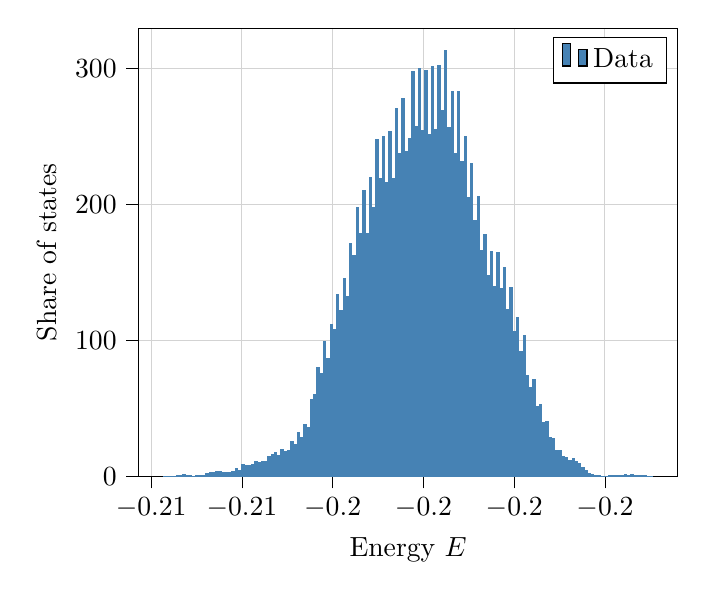
\begin{tikzpicture}

\definecolor{lightgray}{RGB}{211,211,211}
\definecolor{steelblue}{RGB}{70,130,180}

\begin{axis}[
tick align=outside,
tick pos=left,
x grid style={lightgray},
xlabel={Energy \(\displaystyle E\)},
xmajorgrids,
xmin=-0.208285, xmax=-0.196392777777778,
xtick style={color=black},
y grid style={lightgray},
ylabel={Share of states},
ymajorgrids,
ymin=0, ymax=329.294120347803,
ytick style={color=black}
]
\draw[draw=none,fill=steelblue] (axis cs:-0.207744444444444,0) rectangle (axis cs:-0.20767237037037,0.183328204179825);
\addlegendimage{ybar,ybar legend,draw=none,fill=steelblue}
\addlegendentry{Data}

\draw[draw=none,fill=steelblue] (axis cs:-0.20767237037037,0) rectangle (axis cs:-0.207600296296296,0.381933758708117);
\draw[draw=none,fill=steelblue] (axis cs:-0.207600296296296,0) rectangle (axis cs:-0.207528222222222,0.473597860797882);
\draw[draw=none,fill=steelblue] (axis cs:-0.207528222222222,0) rectangle (axis cs:-0.207456148148148,0.611094013932987);
\draw[draw=none,fill=steelblue] (axis cs:-0.207456148148148,0) rectangle (axis cs:-0.207384074074074,1.09996922507895);
\draw[draw=none,fill=steelblue] (axis cs:-0.207384074074074,0) rectangle (axis cs:-0.207312,1.39023888169701);
\draw[draw=none,fill=steelblue] (axis cs:-0.207312,0) rectangle (axis cs:-0.207239925925926,1.90966879354058);
\draw[draw=none,fill=steelblue] (axis cs:-0.207239925925926,0) rectangle (axis cs:-0.207167851851852,1.09996922507895);
\draw[draw=none,fill=steelblue] (axis cs:-0.207167851851852,0) rectangle (axis cs:-0.207095777777778,0.993027772641104);
\draw[draw=none,fill=steelblue] (axis cs:-0.207095777777778,0) rectangle (axis cs:-0.207023703703704,0.687480765674346);
\draw[draw=none,fill=steelblue] (axis cs:-0.207023703703704,0) rectangle (axis cs:-0.20695162962963,1.43607093274197);
\draw[draw=none,fill=steelblue] (axis cs:-0.20695162962963,0) rectangle (axis cs:-0.206879555555556,1.09996922507938);
\draw[draw=none,fill=steelblue] (axis cs:-0.206879555555556,0) rectangle (axis cs:-0.206807481481481,1.34440683065205);
\draw[draw=none,fill=steelblue] (axis cs:-0.206807481481481,0) rectangle (axis cs:-0.206735407407407,2.26104785155205);
\draw[draw=none,fill=steelblue] (axis cs:-0.206735407407407,0) rectangle (axis cs:-0.206663333333333,3.42212647802341);
\draw[draw=none,fill=steelblue] (axis cs:-0.206663333333333,0) rectangle (axis cs:-0.206591259259259,3.42212647802473);
\draw[draw=none,fill=steelblue] (axis cs:-0.206591259259259,0) rectangle (axis cs:-0.206519185185185,4.24710339683262);
\draw[draw=none,fill=steelblue] (axis cs:-0.206519185185185,0) rectangle (axis cs:-0.206447111111111,3.8193375870797);
\draw[draw=none,fill=steelblue] (axis cs:-0.206447111111111,0) rectangle (axis cs:-0.206375037037037,3.08602477036158);
\draw[draw=none,fill=steelblue] (axis cs:-0.206375037037037,0) rectangle (axis cs:-0.206302962962963,3.20824357314695);
\draw[draw=none,fill=steelblue] (axis cs:-0.206302962962963,0) rectangle (axis cs:-0.206230888888889,3.37629442697975);
\draw[draw=none,fill=steelblue] (axis cs:-0.206230888888889,0) rectangle (axis cs:-0.206158814814815,4.29293544787758);
\draw[draw=none,fill=steelblue] (axis cs:-0.206158814814815,0) rectangle (axis cs:-0.206086740740741,6.2637136428107);
\draw[draw=none,fill=steelblue] (axis cs:-0.206086740740741,0) rectangle (axis cs:-0.206014666666667,5.10263501634044);
\draw[draw=none,fill=steelblue] (axis cs:-0.206014666666667,0) rectangle (axis cs:-0.205942592592593,9.42612516491269);
\draw[draw=none,fill=steelblue] (axis cs:-0.205942592592593,0) rectangle (axis cs:-0.205870518518519,8.32615593983695);
\draw[draw=none,fill=steelblue] (axis cs:-0.205870518518519,0) rectangle (axis cs:-0.205798444444444,8.55531619505852);
\draw[draw=none,fill=steelblue] (axis cs:-0.205798444444444,0) rectangle (axis cs:-0.20572637037037,9.48723456630597);
\draw[draw=none,fill=steelblue] (axis cs:-0.20572637037037,0) rectangle (axis cs:-0.205654296296296,11.3969033598502);
\draw[draw=none,fill=steelblue] (axis cs:-0.205654296296296,0) rectangle (axis cs:-0.205582222222222,10.3580435361601);
\draw[draw=none,fill=steelblue] (axis cs:-0.205582222222222,0) rectangle (axis cs:-0.205510148148148,11.1219110535804);
\draw[draw=none,fill=steelblue] (axis cs:-0.205510148148148,0) rectangle (axis cs:-0.205438074074074,11.3663486591492);
\draw[draw=none,fill=steelblue] (axis cs:-0.205438074074074,0) rectangle (axis cs:-0.205366,14.7273657357793);
\draw[draw=none,fill=steelblue] (axis cs:-0.205366,0) rectangle (axis cs:-0.205293925925926,16.423151624449);
\draw[draw=none,fill=steelblue] (axis cs:-0.205293925925926,0) rectangle (axis cs:-0.205221851851852,17.9967187103195);
\draw[draw=none,fill=steelblue] (axis cs:-0.205221851851852,0) rectangle (axis cs:-0.205149777777778,15.6134520559878);
\draw[draw=none,fill=steelblue] (axis cs:-0.205149777777778,0) rectangle (axis cs:-0.205077703703704,19.8911101535111);
\draw[draw=none,fill=steelblue] (axis cs:-0.205077703703704,0) rectangle (axis cs:-0.20500562962963,18.7605862277355);
\draw[draw=none,fill=steelblue] (axis cs:-0.20500562962963,0) rectangle (axis cs:-0.204933555555556,19.5550084458556);
\draw[draw=none,fill=steelblue] (axis cs:-0.204933555555556,0) rectangle (axis cs:-0.204861481481481,26.2464878984117);
\draw[draw=none,fill=steelblue] (axis cs:-0.204861481481481,0) rectangle (axis cs:-0.204789407407407,24.138213550353);
\draw[draw=none,fill=steelblue] (axis cs:-0.204789407407407,0) rectangle (axis cs:-0.204717333333333,32.3727053880875);
\draw[draw=none,fill=steelblue] (axis cs:-0.204717333333333,0) rectangle (axis cs:-0.204645259259259,29.1644618149406);
\draw[draw=none,fill=steelblue] (axis cs:-0.204645259259259,0) rectangle (axis cs:-0.204573185185185,38.4989228777782);
\draw[draw=none,fill=steelblue] (axis cs:-0.204573185185185,0) rectangle (axis cs:-0.204501111111111,36.1767656248189);
\draw[draw=none,fill=steelblue] (axis cs:-0.204501111111111,0) rectangle (axis cs:-0.204429037037037,57.1525676530826);
\draw[draw=none,fill=steelblue] (axis cs:-0.204429037037037,0) rectangle (axis cs:-0.204356962962963,60.7427449849155);
\draw[draw=none,fill=steelblue] (axis cs:-0.204356962962963,0) rectangle (axis cs:-0.204284888888889,80.3894175328844);
\draw[draw=none,fill=steelblue] (axis cs:-0.204284888888889,0) rectangle (axis cs:-0.204212814814815,75.8214897787062);
\draw[draw=none,fill=steelblue] (axis cs:-0.204212814814815,0) rectangle (axis cs:-0.204140740740741,99.2416678626788);
\draw[draw=none,fill=steelblue] (axis cs:-0.204140740740741,0) rectangle (axis cs:-0.204068666666667,87.1572837371922);
\draw[draw=none,fill=steelblue] (axis cs:-0.204068666666667,0) rectangle (axis cs:-0.203996592592593,112.04408745457);
\draw[draw=none,fill=steelblue] (axis cs:-0.203996592592593,0) rectangle (axis cs:-0.203924518518519,108.713625078678);
\draw[draw=none,fill=steelblue] (axis cs:-0.203924518518519,0) rectangle (axis cs:-0.203852444444444,133.722647598834);
\draw[draw=none,fill=steelblue] (axis cs:-0.203852444444444,0) rectangle (axis cs:-0.20378037037037,121.959087830629);
\draw[draw=none,fill=steelblue] (axis cs:-0.20378037037037,0) rectangle (axis cs:-0.203708296296296,145.516762067793);
\draw[draw=none,fill=steelblue] (axis cs:-0.203708296296296,0) rectangle (axis cs:-0.203636222222222,132.454627519924);
\draw[draw=none,fill=steelblue] (axis cs:-0.203636222222222,0) rectangle (axis cs:-0.203564148148148,171.793804666911);
\draw[draw=none,fill=steelblue] (axis cs:-0.203564148148148,0) rectangle (axis cs:-0.203492074074074,162.367679501932);
\draw[draw=none,fill=steelblue] (axis cs:-0.203492074074074,0) rectangle (axis cs:-0.20342,198.131956667346);
\draw[draw=none,fill=steelblue] (axis cs:-0.20342,0) rectangle (axis cs:-0.203347925925926,178.63805762296);
\draw[draw=none,fill=steelblue] (axis cs:-0.203347925925926,0) rectangle (axis cs:-0.203275851851852,210.323282245305);
\draw[draw=none,fill=steelblue] (axis cs:-0.203275851851852,0) rectangle (axis cs:-0.203203777777778,178.867217878185);
\draw[draw=none,fill=steelblue] (axis cs:-0.203203777777778,0) rectangle (axis cs:-0.203131703703704,219.902180913701);
\draw[draw=none,fill=steelblue] (axis cs:-0.203131703703704,0) rectangle (axis cs:-0.20305962962963,198.147234017695);
\draw[draw=none,fill=steelblue] (axis cs:-0.20305962962963,0) rectangle (axis cs:-0.202987555555556,247.630571795995);
\draw[draw=none,fill=steelblue] (axis cs:-0.202987555555556,0) rectangle (axis cs:-0.202915481481481,219.199422797678);
\draw[draw=none,fill=steelblue] (axis cs:-0.202915481481481,0) rectangle (axis cs:-0.202843407407407,250.120779902772);
\draw[draw=none,fill=steelblue] (axis cs:-0.202843407407407,0) rectangle (axis cs:-0.202771333333333,216.296726231497);
\draw[draw=none,fill=steelblue] (axis cs:-0.202771333333333,0) rectangle (axis cs:-0.202699259259259,253.726234584878);
\draw[draw=none,fill=steelblue] (axis cs:-0.202699259259259,0) rectangle (axis cs:-0.202627185185185,219.107758695672);
\draw[draw=none,fill=steelblue] (axis cs:-0.202627185185185,0) rectangle (axis cs:-0.202555111111111,270.485487916984);
\draw[draw=none,fill=steelblue] (axis cs:-0.202555111111111,0) rectangle (axis cs:-0.202483037037037,237.593352617145);
\draw[draw=none,fill=steelblue] (axis cs:-0.202483037037037,0) rectangle (axis cs:-0.202410962962963,278.124163091144);
\draw[draw=none,fill=steelblue] (axis cs:-0.202410962962963,0) rectangle (axis cs:-0.202338888888889,239.380802607899);
\draw[draw=none,fill=steelblue] (axis cs:-0.202338888888889,0) rectangle (axis cs:-0.202266814814815,248.53193546645);
\draw[draw=none,fill=steelblue] (axis cs:-0.202266814814815,0) rectangle (axis cs:-0.202194740740741,298.152769397789);
\draw[draw=none,fill=steelblue] (axis cs:-0.202194740740741,0) rectangle (axis cs:-0.202122666666667,257.545572172057);
\draw[draw=none,fill=steelblue] (axis cs:-0.202122666666667,0) rectangle (axis cs:-0.202050592592593,300.062438191329);
\draw[draw=none,fill=steelblue] (axis cs:-0.202050592592593,0) rectangle (axis cs:-0.201978518518519,254.581766204482);
\draw[draw=none,fill=steelblue] (axis cs:-0.201978518518519,0) rectangle (axis cs:-0.201906444444444,298.611089908239);
\draw[draw=none,fill=steelblue] (axis cs:-0.201906444444444,0) rectangle (axis cs:-0.20183437037037,251.556850835417);
\draw[draw=none,fill=steelblue] (axis cs:-0.20183437037037,0) rectangle (axis cs:-0.201762296296296,301.742946729761);
\draw[draw=none,fill=steelblue] (axis cs:-0.201762296296296,0) rectangle (axis cs:-0.201690222222222,255.376188422497);
\draw[draw=none,fill=steelblue] (axis cs:-0.201690222222222,0) rectangle (axis cs:-0.201618148148148,302.185989889862);
\draw[draw=none,fill=steelblue] (axis cs:-0.201618148148148,0) rectangle (axis cs:-0.201546074074074,269.309131940164);
\draw[draw=none,fill=steelblue] (axis cs:-0.201546074074074,0) rectangle (axis cs:-0.201474,313.613447950288);
\draw[draw=none,fill=steelblue] (axis cs:-0.201474,0) rectangle (axis cs:-0.201401925925926,256.903923457428);
\draw[draw=none,fill=steelblue] (axis cs:-0.201401925925926,0) rectangle (axis cs:-0.201329851851852,283.15041135574);
\draw[draw=none,fill=steelblue] (axis cs:-0.201329851851852,0) rectangle (axis cs:-0.201257777777778,237.318360310875);
\draw[draw=none,fill=steelblue] (axis cs:-0.201257777777778,0) rectangle (axis cs:-0.201185703703704,283.15041135574);
\draw[draw=none,fill=steelblue] (axis cs:-0.201185703703704,0) rectangle (axis cs:-0.20111362962963,231.558799229468);
\draw[draw=none,fill=steelblue] (axis cs:-0.20111362962963,0) rectangle (axis cs:-0.201041555555556,249.815232895805);
\draw[draw=none,fill=steelblue] (axis cs:-0.201041555555556,0) rectangle (axis cs:-0.200969481481481,205.297033980708);
\draw[draw=none,fill=steelblue] (axis cs:-0.200969481481481,0) rectangle (axis cs:-0.200897407407407,230.031064194725);
\draw[draw=none,fill=steelblue] (axis cs:-0.200897407407407,0) rectangle (axis cs:-0.200825333333333,188.278065692681);
\draw[draw=none,fill=steelblue] (axis cs:-0.200825333333333,0) rectangle (axis cs:-0.200753259259259,206.076178848472);
\draw[draw=none,fill=steelblue] (axis cs:-0.200753259259259,0) rectangle (axis cs:-0.200681185185185,166.232849140121);
\draw[draw=none,fill=steelblue] (axis cs:-0.200681185185185,0) rectangle (axis cs:-0.200609111111111,178.500561469757);
\draw[draw=none,fill=steelblue] (axis cs:-0.200609111111111,0) rectangle (axis cs:-0.200537037037037,147.793087269693);
\draw[draw=none,fill=steelblue] (axis cs:-0.200537037037037,0) rectangle (axis cs:-0.200464962962963,165.499536323337);
\draw[draw=none,fill=steelblue] (axis cs:-0.200464962962963,0) rectangle (axis cs:-0.200392888888889,139.665536884384);
\draw[draw=none,fill=steelblue] (axis cs:-0.200392888888889,0) rectangle (axis cs:-0.200320814814815,165.285653418461);
\draw[draw=none,fill=steelblue] (axis cs:-0.200320814814815,0) rectangle (axis cs:-0.200248740740741,138.321130053678);
\draw[draw=none,fill=steelblue] (axis cs:-0.200248740740741,0) rectangle (axis cs:-0.200176666666667,153.766531255888);
\draw[draw=none,fill=steelblue] (axis cs:-0.200176666666667,0) rectangle (axis cs:-0.200104592592593,122.936838252921);
\draw[draw=none,fill=steelblue] (axis cs:-0.200104592592593,0) rectangle (axis cs:-0.200032518518519,139.421099278811);
\draw[draw=none,fill=steelblue] (axis cs:-0.200032518518518,0) rectangle (axis cs:-0.199960444444444,107.155335343108);
\draw[draw=none,fill=steelblue] (axis cs:-0.199960444444444,0) rectangle (axis cs:-0.19988837037037,117.024503668122);
\draw[draw=none,fill=steelblue] (axis cs:-0.19988837037037,0) rectangle (axis cs:-0.199816296296296,92.4279696073643);
\draw[draw=none,fill=steelblue] (axis cs:-0.199816296296296,0) rectangle (axis cs:-0.199744222222222,103.809595616826);
\draw[draw=none,fill=steelblue] (axis cs:-0.199744222222222,0) rectangle (axis cs:-0.199672148148148,74.3854188459928);
\draw[draw=none,fill=steelblue] (axis cs:-0.199672148148148,0) rectangle (axis cs:-0.199600074074074,65.4940009432427);
\draw[draw=none,fill=steelblue] (axis cs:-0.199600074074074,0) rectangle (axis cs:-0.199528,71.6354957832668);
\draw[draw=none,fill=steelblue] (axis cs:-0.199528,0) rectangle (axis cs:-0.199455925925926,52.0957646877871);
\draw[draw=none,fill=steelblue] (axis cs:-0.199455925925926,0) rectangle (axis cs:-0.199383851851852,53.0124057086662);
\draw[draw=none,fill=steelblue] (axis cs:-0.199383851851852,0) rectangle (axis cs:-0.199311777777778,40.3780369706221);
\draw[draw=none,fill=steelblue] (axis cs:-0.199311777777778,0) rectangle (axis cs:-0.199239703703704,40.4697010726965);
\draw[draw=none,fill=steelblue] (axis cs:-0.199239703703704,0) rectangle (axis cs:-0.19916762962963,29.1797391652889);
\draw[draw=none,fill=steelblue] (axis cs:-0.19916762962963,0) rectangle (axis cs:-0.199095555555556,28.2019887430073);
\draw[draw=none,fill=steelblue] (axis cs:-0.199095555555556,0) rectangle (axis cs:-0.199023481481481,19.6772272486346);
\draw[draw=none,fill=steelblue] (axis cs:-0.199023481481481,0) rectangle (axis cs:-0.198951407407407,19.1425199864508);
\draw[draw=none,fill=steelblue] (axis cs:-0.198951407407407,0) rectangle (axis cs:-0.198879333333333,14.7884751371726);
\draw[draw=none,fill=steelblue] (axis cs:-0.198879333333333,0) rectangle (axis cs:-0.198807259259259,14.3912640281163);
\draw[draw=none,fill=steelblue] (axis cs:-0.198807259259259,0) rectangle (axis cs:-0.198735185185185,12.3593764317947);
\draw[draw=none,fill=steelblue] (axis cs:-0.198735185185185,0) rectangle (axis cs:-0.198663111111111,13.3829589051273);
\draw[draw=none,fill=steelblue] (axis cs:-0.198663111111111,0) rectangle (axis cs:-0.198591037037037,11.0760790025354);
\draw[draw=none,fill=steelblue] (axis cs:-0.198591037037037,0) rectangle (axis cs:-0.198518962962963,9.76222687257571);
\draw[draw=none,fill=steelblue] (axis cs:-0.198518962962963,0) rectangle (axis cs:-0.198446888888889,6.78314355465615);
\draw[draw=none,fill=steelblue] (axis cs:-0.198446888888889,0) rectangle (axis cs:-0.198374814814815,5.07208031564184);
\draw[draw=none,fill=steelblue] (axis cs:-0.198374814814815,0) rectangle (axis cs:-0.198302740740741,2.78047776339402);
\draw[draw=none,fill=steelblue] (axis cs:-0.198302740740741,0) rectangle (axis cs:-0.198230666666667,2.01661024597886);
\draw[draw=none,fill=steelblue] (axis cs:-0.198230666666667,0) rectangle (axis cs:-0.198158592592593,1.42079358239365);
\draw[draw=none,fill=steelblue] (axis cs:-0.198158592592593,0) rectangle (axis cs:-0.198086518518518,0.916641020899127);
\draw[draw=none,fill=steelblue] (axis cs:-0.198086518518518,0) rectangle (axis cs:-0.198014444444444,0.320824357314818);
\draw[draw=none,fill=steelblue] (axis cs:-0.198014444444444,0) rectangle (axis cs:-0.19794237037037,0.473597860797882);
\draw[draw=none,fill=steelblue] (axis cs:-0.19794237037037,0) rectangle (axis cs:-0.197870296296296,0.824976918809532);
\draw[draw=none,fill=steelblue] (axis cs:-0.197870296296296,0) rectangle (axis cs:-0.197798222222222,1.2221880278655);
\draw[draw=none,fill=steelblue] (axis cs:-0.197798222222222,0) rectangle (axis cs:-0.197726148148148,1.09996922507938);
\draw[draw=none,fill=steelblue] (axis cs:-0.197726148148148,0) rectangle (axis cs:-0.197654074074074,1.17635597682055);
\draw[draw=none,fill=steelblue] (axis cs:-0.197654074074074,0) rectangle (axis cs:-0.197582,1.2221880278655);
\draw[draw=none,fill=steelblue] (axis cs:-0.197582,0) rectangle (axis cs:-0.197509925925926,1.74161793970901);
\draw[draw=none,fill=steelblue] (axis cs:-0.197509925925926,0) rectangle (axis cs:-0.197437851851852,1.06941452438232);
\draw[draw=none,fill=steelblue] (axis cs:-0.197437851851852,0) rectangle (axis cs:-0.197365777777778,1.92494614388891);
\draw[draw=none,fill=steelblue] (axis cs:-0.197365777777778,0) rectangle (axis cs:-0.197293703703704,0.947195721595765);
\draw[draw=none,fill=steelblue] (axis cs:-0.197293703703704,0) rectangle (axis cs:-0.19722162962963,1.23746537821382);
\draw[draw=none,fill=steelblue] (axis cs:-0.19722162962963,0) rectangle (axis cs:-0.197149555555556,1.32912948030425);
\draw[draw=none,fill=steelblue] (axis cs:-0.197149555555556,0) rectangle (axis cs:-0.197077481481481,0.962473071944084);
\draw[draw=none,fill=steelblue] (axis cs:-0.197077481481481,0) rectangle (axis cs:-0.197005407407407,0.274992306269844);
\draw[draw=none,fill=steelblue] (axis cs:-0.197005407407407,0) rectangle (axis cs:-0.196933333333333,0.106941452438232);
\end{axis}

\end{tikzpicture}

\end{figure}

\begin{figure}
\centering
\graphicspath{{../../Plots/}}
% This file was created with tikzplotlib v0.10.1.
\begin{tikzpicture}

\definecolor{lightgray}{RGB}{211,211,211}

\begin{axis}[
tick align=outside,
tick pos=left,
x grid style={lightgray},
xmajorgrids,
xmin=-0.5, xmax=19.5,
xtick style={color=black},
y dir=reverse,
y grid style={lightgray},
ymajorgrids,
ymin=-0.5, ymax=19.5,
ytick style={color=black}
]
\addplot graphics [includegraphics cmd=\pgfimage,xmin=-0.5, xmax=19.5, ymin=19.5, ymax=-0.5] {../../Plots/High_temp_state_10000-002.png};
\end{axis}

\end{tikzpicture}

\end{figure}


\newpage
\section*{Bibliography}
%\nocite{*}
%Main source
%\printbibliography[heading=none, keyword={main}]
%\noindent Other sources
\printbibliography[heading=none, keyword={secondary}]

\end{document}
